% ============================================================================
% Figure 2: Stratified performance by grid size N and removal ratio r.
% Grouped bars of valid-solution rate (%) per solver family across six strata.
% Data source: paper/tables/table3_difficulty_stratification.csv.
% SAT attempted counts reflect 7 configs minus predeclared exclusions at N=81
% (40 per stratum); CP-SAT and Backtracking attempted = 20 per stratum.
% Valid counts: SAT [140,140,13,138,0,0]; CP-SAT [20,20,4,20,0,0];
% Backtracking [20,20,0,0,0,0] across strata
%   (N9r0.5,N9r0.9,N36r0.5,N36r0.9,N81r0.5,N81r0.9).
% Excluded/non-attempted runs are shown as annotations; no bar is drawn for
% missing combinations.
% ============================================================================
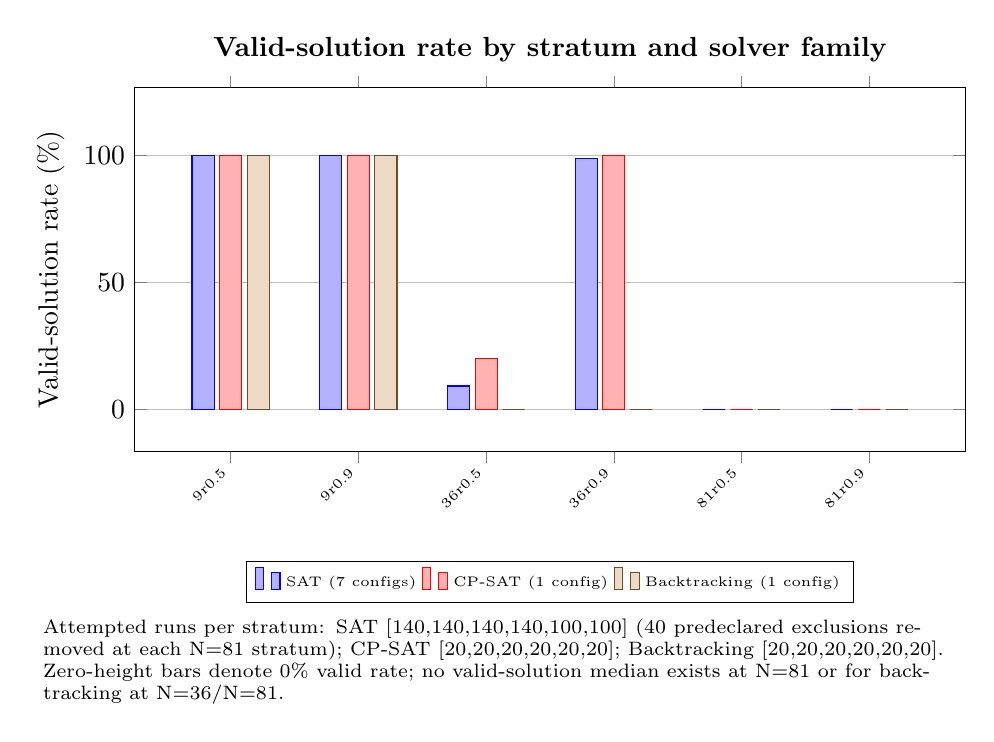
\begin{tikzpicture}
\begin{axis}[
  ybar, bar width=0.28cm,
  symbolic x coords={
    9r0.5,9r0.9,36r0.5,36r0.9,81r0.5,81r0.9
  },
  xtick=data,
  xticklabel style={font=\tiny, rotate=45, anchor=east},
  x tick label style={/pgf/number format/1000 sep={}},
  ylabel={Valid-solution rate (\%)},
  ymin=0, ymax=110,
  ymajorgrids=true,
  enlargelimits=0.15,
  legend style={at={(0.5,-0.30)}, anchor=north, legend columns=3, font=\tiny},
  width=\textwidth, height=6.2cm,
  title style={font=\bfseries},
  title={Valid-solution rate by stratum and solver family},
]
% SAT (pooled 7 configs)
\addplot coordinates {
  (9r0.5,100.00) (9r0.9,100.00) (36r0.5,9.29) (36r0.9,98.57) (81r0.5,0.00) (81r0.9,0.00)
};
\addlegendentry{SAT (7 configs)}
% CP-SAT
\addplot coordinates {
  (9r0.5,100.00) (9r0.9,100.00) (36r0.5,20.00) (36r0.9,100.00) (81r0.5,0.00) (81r0.9,0.00)
};
\addlegendentry{CP-SAT (1 config)}
% Backtracking
\addplot coordinates {
  (9r0.5,100.00) (9r0.9,100.00) (36r0.5,0.00) (36r0.9,0.00) (81r0.5,0.00) (81r0.9,0.00)
};
\addlegendentry{Backtracking (1 config)}
\end{axis}

% Annotation of attempted / excluded counts (placed below axis as a note)
\node[align=left, font=\scriptsize, text width=0.95\textwidth] at (current bounding box.south) [yshift=-0.75cm] {
  Attempted runs per stratum: SAT [140,140,140,140,100,100] (40 predeclared exclusions removed at each N=81 stratum);
  CP-SAT [20,20,20,20,20,20]; Backtracking [20,20,20,20,20,20].
  Zero-height bars denote 0\% valid rate; no valid-solution median exists at N=81 or for backtracking at N=36/N=81.
};
\end{tikzpicture}
